\section*{Appendix 16}
\label{sec:app16}
Mathematically, the Levenshtein distance between two strings a,b of length |a| and |b| respectively is given by lev a,b(|a|,|b|) where
\begin{figure}[ht!]
  \centering
  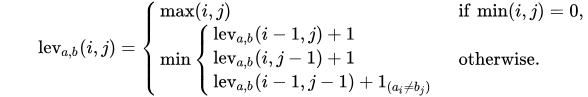
\includegraphics[width=0.9\textwidth]{figures/levenshtein.png}
  \label{fig:levenshtein}
\end{figure}
\par

Where 1(ai$\neq$ bj) is equal to 0 when ai = bj and equal to 1 otherwise, and leva,b(i,j) is the distance between the first i characters of a and the first j characters of b.
